\section{Ejercicio 2}

\subsection{Introducción a la G.U.I.}

Se realizó una aplicación de interfaz gráfica, la cual permite representar Diagramas de BODE de fase y amplitud para una o múltiples funciones transferencias, en simultaneo o no, en gráficas separadas o no, ingresadas por el usuario mediante distintas fuentes:

\begin{itemize}
    \item Ingreso Manual de los coeficientes del cociente de polimonios de la función de transferencia.
    \item Carga de archivo con outputs de simulaciones del software LT Spice.
    \item Carga de archivo de extensión CSV con métricas de mediciones. 

\end{itemize}

\subsection{Manual de Uso}

Se enumerarán todas las funcionalidades disponibles que incluye la Plot Tool del presente grupo, se explicará su funcionamiento y cómo operar cada una de ellas:

\subsubsection{Etiquetas para Ejes $X$ e $Y$ de los Diagramas de BODE}

Mediante esta funcionalidad, se podrá ingresar en cada cuadro de texto las etiquetas deseadas para los Ejes X e Y de cada diagrama de BODE de manera independiente. 

Para utilizar dicha función, basta con ingresar el texto deseado para ser representado en los campos $Etiqueta Eje X$ o $Etiqueta Eje Y$ y seleccionar mediante $H(S)$ o $\phi$ si esas etiquetas aplicarán para el Diagrama Bode de Magnitud, Fase o Ambos.

En el caso de querer eliminar las etiquetas ya añadidas a dichos ejes, el usuario debe dejar los campos $Etiqueta Eje X$ o $Etiqueta Eje Y$  en blanco según sea el caso y seleccionar sobre qué gráfico se desea eliminar las etiquetas presionando $H(S)$ o $\phi$.

% INSERTAR IMAGEN DE ETIQUETA
\begin{figure}[h]
	\centering
	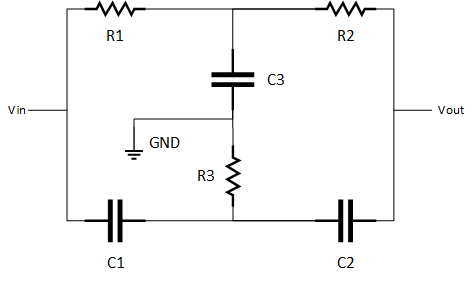
\includegraphics[scale=1]{../EJ1/circuito.png}
	\caption{Filtro Notch Pasivo}
	\label{ej1cir}
\end{figure}

\subsubsection{Grafico de Diagramas de BODE mediante ingreso manual}


Se podrá ingresar una función de transferencia representada como cociente de polinomios según la forma:

$$H(S) = \frac{aS^n + bS^{n-1}+ ... +cS^{n-i}}{eS^m + fS^{m-1}+ ... +gS^{m-j}} $$

Para ello, se debe seleccionar la opción $H(S)$. Se deberán ingresar los valores de los coeficientes del polinomio del numerador y denominador correspondientemente separados por ",". El primer valor ingresado tanto para el numerador como el denominador representarán el coeficiente de la potencia de mayor grado del polinomio y los siguientes elementos representarán los de grado $n-1, n -2 , ... , n-m$. Deberán ingresarse tantos elementos como coeficientes haya en el polinomio que se quiera representar. En los casos donde haya coeficientes nulos, se deberán ingresar $0$ como elemento.
Es decir, que si queremos representar un polinomio de grado $n$ y algunos o todos los coeficientes de las potencias de grado menor son nulas, indefectiblemente, el usuario deberá ingresar $0$ para poder alcanzar el grado deseado del polinomio.

Además de ello, se podrá ingresar un $Nombre$ para la función de transferencia que será utilizado como etiqueta en el gráfico una vez que se proceda a realizar los diagramas aceptado el proceso por el usuario.

\paragraph{Ejemplo 1}

Si el input de los campos $Numerador$ o $Denominador$ es "1,1,1" esto representará el polinomio  $$H(S) = S^2 + S + 1 $$

\paragraph{Ejemplo 2}

Si el input de los campos $Numerador$ o $Denominador$ es "1,0,1,0,1" esto representará el polinomio  $$H(S) = S^4 + S^2 + 1 $$

\paragraph{Ejemplo 3}

Si se desea representar $$H(S) = \frac{1}{S^2 + 1} $$el input de los campos $Numerador$ y $Denominador$ será "1" y "1,0,1" respectivamente.

Para hacer más amigable la interfaz, una vez seleccionado $Ingresar$ se representarán los datos ingresados por el usuario de la siguiente manera:

$$H(S) = \frac{aS^n + bS^{n-1}+ ... +cS^{n-i}}{eS^m + fS^{m-1}+ ... +gS^{m-j}} $$

En caso de que la función $H(S)$ no coincida con la función transferencia que se desea ingresar, simplemente se puede seleccionar $Volver$ para modificar nuevamente los elementos para el $Numerador$ y/o $Denominador$. 
Una vez validados los datos en la sección de previsualización se podrá seleccionar $Aceptar$ para obtener los diagramas de BODE de la función ingresada.

IMAGEN DE GRAFICO

\subsubsection{Gráfico de Diagramas de BODE mediante carga de archivo de LTSpice}

Se podrá ingresar una función de transferencia calculada en base a archivos generados mediante simulaciones realizadas con el software LTSpice.

Para ello, se debe seleccionar la opción $SPICE$ y seleccionar $Buscar$ para localizar el archivo correspondiente dentro de los directorios del sistema operativo. 
Una vez seleccionado, la aplicación procesará el archivo, y si el formato del mismo es válido procederá a realizar los Diagramas de BODE correspondientes.

IMAGEN DE LT SPICE

\subsubsection{Gráfico de Diagramas de BODE mediante carga de archivos de extensión CSV}

Se podrá ingresar una función de transferencia calculada en base a métricas tomadas mediante mediciones reales encapsuladas en un archivo de extensión CSV.

Para ello, se debe seleccionar la opción $Mediciòn$ N y seleccionar $Buscar$ para localizar el archivo correspondiente dentro de los directorios del sistema operativo. 
Una vez seleccionado, la aplicación procesará el archivo, y si el formato del mismo es válido procederá a realizar los Diagramas de BODE correspondientes.

IMAGEN DE CSV

\subsubsection{Representación de Diagramas de BODE de varias funciones transferencia en simultaneo}

Se podrá graficar más de una función de transferencia superpuesta en el mismo gráfico tanto para el Diagrama de BODE de Magnitud como de Fase.
Para ello, bastará con que el usuario repita el proceso mencionado en las secciones $2.2.2$, $2.2.3$ o $2.2.4$ habiendo ingresado previamente al menos una función transferencia.

Al repetir dichos procesos, se obtendrán como resultado curvas superpuestas en los mismos gráficos representando cada una de ellas a las funciones de transferencia ingresadas. 
Cabe destacar que no hay límite para la cantidad de funciones superpuestas en un mismo gráfico, pero se deberá tener en cuenta que los gráficos se adaptarán para mostrar todas las curvas apropiadamente.

IMAGEN CON TODO

\subsubsection{Representación de Diagramas de BODE de un solo tipo}

Se enunciará por Tipo a las distintas formas de ingreso de funciones transferencia de la aplicación, nombrando a ellas nuevamente como:

\begin{itemize}
    \item Ingreso Manual de los coeficientes del cociente de polimonios de la función de transferencia.
    \item Carga de archivo con outputs de simulaciones del software LT Spice.
    \item Carga de archivo de extensión CSV con métricas de mediciones. 

\end{itemize}

Si se han ingresado funciones de transferencia de al menos dos tipos diferentes, se podrá utilizar esta funcionalidad para ocultar el tipo de función transferencia que el usuario desea remover de los Diagramas de BODE.
Esto implica que las curvas de un determinado tipo, serán removidas de los gráficos pudiendo ellas volver a ser graficadas.

Para ello, se debe seleccionar el checkbox $Incluir$ que se encuentre por debajo de cada opción, $H(S)$, $SPICE$ o $Medicion$. En caso de que un checkbox no esté seleccionado, implicará que todas las funciones transferencia de dicho tipo no sean incluidas en los diagramas. 
Se podrá seleccionar/desseleccionar uno, dos o los tres tipos con los efectos correspondientes sobre los gráficos.

\subsubsection{Eliminar los Diagramas de BODE de todas las funciones transferencia}

Para borrar todas las curvas correspondientes a cada función de transferencia para ambos Diagramas de Bode, independientemente del tipo, se podrá seleccionar $Borrar Todo$ sin posibilidad de deshacer esta acción. 

Es importante notar que en caso de que se desee remover temporalmente todas las curvas, pudiendo recuperarlas posteriormente, se podrá utilizar el método descripto en la sección anterior.

\subsubsection{Modos de Representación de Diagramas de BODE}

A efectos de poder obtener herramientas para una mayor capacidad de análisis, se podrán representar los Diagramas BODE de Fase y Amplitud sobre el mismo gráfico. 
Para ello, se debe chequear la opción $Plotear en el mismo gráfico$.

Una vez seleccionada dicha opción aplican todas las mismas funcionalidades mencionadas en las secciones previas con las siguientes diferencias:

\begin{itemize}
    \item \underline{Dos Gráficos:} Un gráfico para el Diagrama de BODE de Amplitud y otro para el Diagrama de BODE de Fase. Ambos gráficos se podrán Guardar por separado.
    \item \underline{Un Gráfico:} Un solo Diagrama de BODE con las representaciones de Fase y Amplitud, donde las curvas de fase estarán representadas con líneas punteadas.

\end{itemize}

